% Chapter 2

\chapter{MicroRNAs and their importance in living beings} % Main chapter title

\label{Chapter2} % For referencing the chapter elsewhere, use \ref{Chapter2} 

%----------------------------------------------------------------------------------------

\section{What are microRNAs?}
MicroRNAs (abbreviated miRNAs) are a family of $\approx 22$-nucleotide small non-coding RNAs that regulates gene expression at the post-transcriptional level \cite{mirna_intro}. This means that they act by binding to partially complementary sites on target genes, which had been previously transcribed from the DNA of the cell, to induce cleavage or repression of productive translation, preventing this way the target gene to be able to exit the cell and start the translational process that produces peptides and proteins.

\begin{figure}[hbt!]
	\centering
	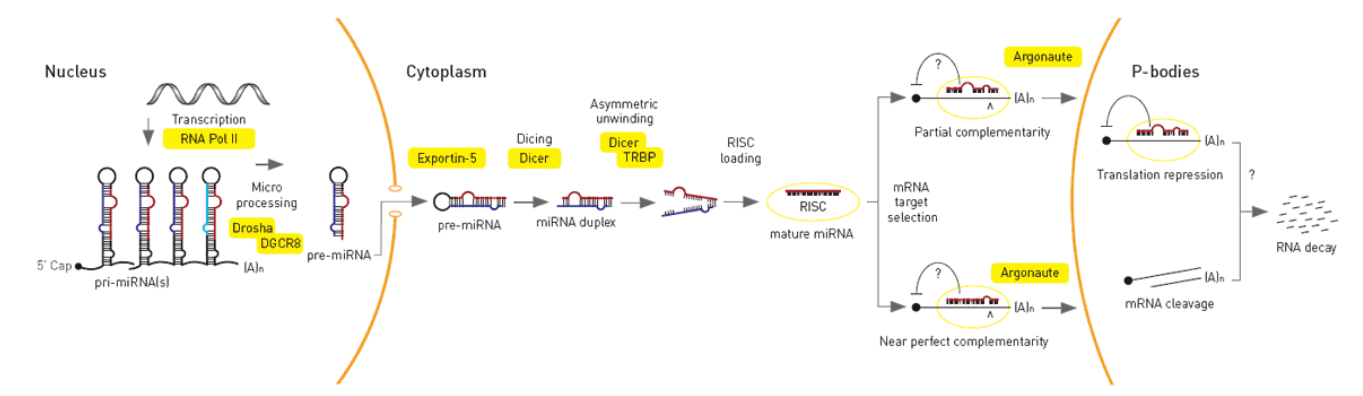
\includegraphics[width=1.0\textwidth]{Figures/mirna_genesis}
	\caption{MiRNAs genesis and functionalities}
	\label{fig:mirna_genesis}
\end{figure}

\subsection{Transcription and processing of miRNAs}
As shown in figure \ref{fig:mirna_genesis} miRNAs genes are transcribed by the RNA polymerase II as as large primary transcripts (pri-miRNA) that are processed by a protein complex containing the enzyme Drosha, to form an approximately 70 nucleotide precursor miRNA (pre-miRNA). This precursor is subsequently transported to the cytoplasm where it is processed by a second enzyme, called DICER, to form a mature miRNA of approximately 22 nucleotides. The mature miRNA is then incorporated into a ribonuclear particle to form the RNA-induced silencing complex, RISC, which mediates gene silencing.

It's important to note that, generally, only one of the two strands of the stem loop is incorporated into the silencing process, and it's selected on the basis of its thermodynamic instability and weaker base-pairing on the 5' end relative to the other strand. The latter, called the passenger strand due to its lower levels in the steady state, is usually denoted with an asterisk (*) and is normally degraded. However, in some cases, both strands of the duplex are viable and become functional miRNAs that target different mRNA populations. (see figure \ref{fig:mirna_stems})

\begin{figure}[hbt!]
	\centering
	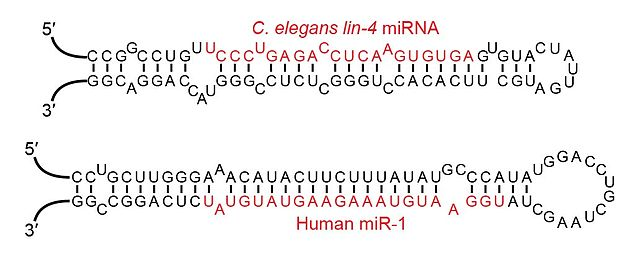
\includegraphics[width=1.0\textwidth]{Figures/mirna_stems}
	\caption{Examples of miRNA stem-loops. In red is shown the mature miRNA}
	\label{fig:mirna_stems}
\end{figure}

\subsection{RNA-induced silencing complex (RISC)}
As mentioned before the mature miRNA is part of an active RNA-induced silencing complex (RISC). This process represents their main functionality in both animals and plants. 
The RISC it is a key process in gene silencing and can act in two different ways as depicted in the right-hand side of picture \ref{fig:mirna_genesis}: via mRNA degradation or by preventing mRNA translation. It has been demonstrated that given complete complementarity between the miRNA and target mRNA sequence, Ago2 can cleave the mRNA and lead to direct mRNA degradation. In the presence of only partial complementarity instead, silencing is achieved by preventing translation \cite{cleavage}.
 
%----------------------------------------------------------------------------------------

\section{Why are they important?}
MiRNAs are particularly abundant in many mammalian cell types and appear to target about 60\% of the genes of humans and other mammals \cite{conserved_pairing}.

Many miRNAs are evolutionarily conserved, which implies that they have important biological functions \cite{conserved_pairing}. For example, 90 families of miRNAs have been conserved since at least the common ancestor of mammals and fish, and most of these conserved miRNAs have important functions.

The discovery of the first miRNA over 20 years ago has ushered in a new era in molecular biology. There are now over 2000 miRNAs that have been discovered in humans and it is believed that they collectively regulate two third of the genes in the genome.

The repressive action of miRNAs has a huge impact on many biological processes such as cell cycle control and several developmental and physiological processes including stem cell differentiation, cardiac and skeletal muscle development, neurogenesis, insulin secretion, cholesterol metabolism, aging, immune responses and viral replication. \cite{mirna_annotation}

In addition to their important roles in healthy individuals, microRNAs have also been implicated in a number of diseases including a broad range of cancers, heart and neurological diseases.  In fact it has been discovered that their expression patterns  are highly specific in respect to external stimuli, developmental stage or tissue and this can be used to diagnose diseases in which the expression levels of miRNAs are known to change considerably \cite{computational_methods}. Consequently, miRNAs are intensely studied as candidates for clinical diagnosis and predictors of drug response \cite{mirna_diseases}.

\section{Why miRNAs target prediction is a difficult task?}
MiRNA's targeting is a complex mechanism, yet not fully understood. This process involves the generation of complex regulatory networks and understanding mechanisms and functions of these networks requires systematic experimental investigation. In an ideal world it would be possible to experimentally validate the targeting set of every miRNA, but the cost and the time needed for the verification make miRNA studies still depending on computational predictions to complement experimental data.

The apparent complementarity between miRNA and its target could be seen as an advantage
for computational analysis; however, other features of miRNA-UTRs association make matters more complicated. The usual sequence alignment algorithms assume longer sequences than the  20-23nt of miRNAs. This short length makes ranking and scoring of targets very difficult as statistical techniques for sequence matching require longer sequences to be significant. Besides, binding sites actually consist of regions of complementarity, bulges and mismatches. Hence, complementarity alone is not sufficient to identify functional targets.  

Recent studies \cite{common_features} \cite{computational_methods} reveal that a single miRNA can bind to many different genes. On average, each miRNA has interactions with over $200$ mRNAs and these genes may accommodate tens of  different site locations along their sequence, however, not all these interactions give origin to a functional binding site: the same miRNA:mRNA pair may create a bond which is functional in a certain tissue but not inside another cell type. 

Besides, environmental conditions and other external factors  may also contribute to binding sites functionality as described in \cite{efficient_use_accessibility}.

All these circumstances make identification of miRNA targets a very challenging task that must be carefully tackled in order to have a better understanding of their role in the gene silencing complex. 
